\setcounter{chapter}{1}
\chapter{ЧИСЛЕННОЕ МОДЕЛИРОВАНИЕ И ИССЛЕДОВАНИЕ ВОЗМОЖНОСТЕЙ РЕГРЕССИОННОГО АНАЛИЗА ДЛЯ ИДЕНТИФИКАЦИИ НЕЛИНЕЙНЫХ ПРОЦЕССОВ}
\label{chap:chislennoe-modelirovanie-i-issledovanie-vozmozhnostei-regressionnogo-analiza-dlya-identifikatsii-nelineinyh-protsessov}

\section{Постановка задачи и методология вычислительного эксперимента}
\label{sec:postanovka-zadachi-i-metodologiya-vychislitelnogo-eksperimenta}

\subsection{Цель и гипотеза вычислительного эксперимента}
\label{sec:tsel-i-gipoteza-vychislitelnogo-eksperimenta}

Цель данной главы состоит в том, чтобы проверить гипотезу в рамках вычислительного эксперимента: в каких режимах линейный регрессионный анализ способен правильно читать структуру детерминированного нелинейного процесса, а в каких режимах высокий fit начинает маскировать ложные лаги, вырождение окна или потерю прогностической устойчивости.

Вычислительный эксперимент проводится на синтетических траекториях, где закон генерации данных задан заранее. Это позволяет оценивать результаты эконометрического анализа в контролируемых условиях, сопоставляя найденную регрессионную структуру с истинным механизмом динамики.

\subsection{Три семейства исследуемых моделей}
\label{sec:tri-semeistva-issleduemyh-modelei}

В работе рассматриваются три типа дискретных отображений, задающих разные варианты реакции системы на ограничение роста. Во всех моделях \(K=1\).

\textbf{1. Базовая модель (мгновенная реакция)}

\[
X_{n+1} = X_n + A X_n (K - X_n)
\]

Темп прироста определяется только текущим состоянием \(X_n\). Истинная структура памяти отсутствует.

\textbf{2. Модель с запаздыванием}

\[
X_{n+1} = X_n + g X_n (K - X_{n-1})
\]

Темп прироста зависит от предыдущего состояния \(X_{n-1}\). Истинная структура содержит лаг 1.

\textbf{3. Смешанная модель}

\[
X_{n+1} = X_n + q X_n (K - X_n - \gamma X_{n-1})
\]

Динамика определяется одновременно текущим уровнем и лагом 1. Это наиболее общий случай, где возможна конкуренция факторов и усиление мультиколлинеарности.

\subsection{Что именно сравнивается}
\label{sec:chto-imenno-sravnivaetsya}

Для каждой модели генерируются траектории в нескольких режимах: от устойчивого роста до колебаний, границы хаоса и развитого динамического хаоса. Далее на этих траекториях строятся регрессионные модели для темпа прироста

\[
\omega_{n+1} = \frac{X_{n+1} - X_n}{X_n},
\]

где в качестве предикторов выступают текущий уровень и лаги ряда. Сравниваются:

\begin{enumerate}
\def\labelenumi{\arabic{enumi}.}
\tightlist
\item
  качество подгонки регрессионной модели;
\item
  способность метода выделить истинные структурные переменные;
\item
  склонность метода включать ложные лаги;
\item
  устойчивость краткосрочного и итеративного прогноза;
\item
  поведение оценок на длинных траекториях и на коротких окнах.
\end{enumerate}

\subsection{Метрики качества и критерии интерпретации}
\label{sec:metriki-kachestva-i-kriterii-interpretatsii}

В качестве основных показателей используются:

\begin{enumerate}
\def\labelenumi{\arabic{enumi}.}
\tightlist
\item
  \(R^2\) и adjusted \(R^2\) как меры локального качества подгонки;
\item
  знаки и величины коэффициентов \(B\);
\item
  стандартизированные коэффициенты \(\beta\) для ранжирования факторов;
\item
  частота ложных лагов и доля правильного восстановления структуры;
\item
  устойчивость прогноза при итеративном продолжении траектории;
\item
  признаки вырождения окна: малая дисперсия, коллинеарность, исчезновение сигнала.
\end{enumerate}

Успех метода в данной главе понимается не как получение максимального fit само по себе, а как совпадение статистического вывода с истинной структурой модели. Неуспехом считается ситуация, когда регрессия демонстрирует высокое качество подгонки, но:

\begin{enumerate}
\def\labelenumi{\arabic{enumi}.}
\tightlist
\item
  выбирает ложные лаги;
\item
  теряет истинную переменную;
\item
  становится неустойчивой на коротких окнах;
\item
  даёт формально хорошее, но содержательно пустое прогнозное продолжение.
\end{enumerate}

\subsection{Дизайн вычислительного эксперимента}
\label{sec:dizain-vychislitelnogo-eksperimenta}

Единый протокол главы включает четыре шага.

\begin{enumerate}
\def\labelenumi{\arabic{enumi}.}
\tightlist
\item
  Генерация траекторий для выбранных параметров и режимов.
\item
  Фазовая диагностика динамики.
\item
  Построение регрессионных моделей \texttt{ENTER} и \texttt{STEPWISE}, а в дополнительных экспериментах также альтернативных диагностических контуров.
\item
  Сравнение полученной регрессионной структуры с истинным законом динамики и анализ прогностической устойчивости.
\end{enumerate}

Краткий паспорт эксперимента приведён в таблице.

{\def\LTcaptype{none} % do not increment counter
\begin{longtable}[]{@{}
  >{\raggedright\arraybackslash}p{(\linewidth - 8\tabcolsep) * \real{0.2000}}
  >{\raggedright\arraybackslash}p{(\linewidth - 8\tabcolsep) * \real{0.2000}}
  >{\raggedright\arraybackslash}p{(\linewidth - 8\tabcolsep) * \real{0.2000}}
  >{\raggedright\arraybackslash}p{(\linewidth - 8\tabcolsep) * \real{0.2000}}
  >{\raggedright\arraybackslash}p{(\linewidth - 8\tabcolsep) * \real{0.2000}}@{}}
\toprule\noalign{}
\begin{minipage}[b]{\linewidth}\raggedright
Модель
\end{minipage} & \begin{minipage}[b]{\linewidth}\raggedright
Истинная структура
\end{minipage} & \begin{minipage}[b]{\linewidth}\raggedright
Основные режимы
\end{minipage} & \begin{minipage}[b]{\linewidth}\raggedright
Ожидание от регрессии
\end{minipage} & \begin{minipage}[b]{\linewidth}\raggedright
Основной риск ошибки
\end{minipage} \\
\midrule\noalign{}
\endhead
\bottomrule\noalign{}
\endlastfoot
Базовая & только \(X_n\) & устойчивый рост, колебания, хаос & выделение текущего уровня без ложной памяти & принятие цикличности за глубокую память \\
Запаздывающая & доминирует \(X_{n-1}\) & рост, затухающие колебания, бифуркация, хаос & выделение лага 1 как ключевого фактора & потеря истинного лага из-за шума и коллинеарности \\
Смешанная & совместно \(X_n\) и \(X_{n-1}\) & устойчивость, цикл, хаос, режимы при \(\gamma<0\) & восстановление конкурирующих факторов и их знаков & ложная подмена структуры дальними лагами \\
\end{longtable}
}

Таким образом, глава 2 строится как последовательная проверка того, где линейная регрессия действительно восстанавливает структуру нелинейного процесса, а где она должна использоваться только как локальный диагностический инструмент.

\section{Описание базовой модели и сценариев эксперимента}
\label{sec:opisanie-bazovoi-modeli-i-stsenariev-eksperimenta}

В данном подразделе рассматривается базовое логистическое отображение

\[
X_{n+1} = X_n + A X_n (K - X_n), \qquad K=1,
\]

в котором истинная структура темпа прироста определяется только текущим состоянием \(X_n\). Для проверки регрессионного аппарата выбраны пять сценариев: \(AK=0.8\), \(AK=1.5\), \(AK=2.2\), \(AK=2.52\) и \(AK=2.8\). Они охватывают устойчивое равновесие, цикл и развитый хаос.

\subsection{Устойчивый режим}
\label{sec:ustoichivyi-rezhim}

Сценарии \(AK=0.8\) и \(AK=1.5\) дают близкий по смыслу результат, поэтому их удобно рассматривать вместе. В обоих случаях траектория сходится к стационарному состоянию, а фазовый портрет согласуется с детерминированной природой процесса и сохраняет параболическую форму \(X_{n+1}=f(X_n)\).

Для этих режимов регрессия работает корректно: метод \texttt{STEPWISE} выделяет только текущий уровень \(X_n\), коэффициент детерминации равен \(R^2 \approx 1\), а оценка влияния \(X_n\) совпадает с теоретическим значением в пределах вычислительной точности. Итеративный прогноз также остаётся устойчивым и на рассматриваемом горизонте практически не расходится с истинной траекторией.

Следовательно, в устойчивом режиме линейная регрессия действительно способна восстановить линейную структуру темпа прироста и не создаёт ложной памяти.

\subsection{Циклический режим}
\label{sec:tsiklicheskii-rezhim}

При \(AK=2.2\) система переходит к устойчивому циклу периода 2, а при \(AK=2.52\) --- к более сложному циклу на границе хаоса. Для регрессионного анализа это принципиально иной класс ситуаций: качество подгонки остаётся очень высоким, но структура модели начинает искажаться.

В режиме \(AK=2.2\) алгоритм \texttt{STEPWISE} выбирает не только \(X_n\), но и \(Lag_2\). Содержательно это ложный результат: уравнение не содержит зависимости от второго лага, а его появление вызвано тем, что в цикле периода 2 значения \(X_n\) и \(X_{n-2}\) почти совпадают. В режиме \(AK=2.52\) эффект усиливается: в модель попадают \(Lag_4\) и статистические дубли более дальних лагов. Тем самым высокая мультиколлинеарность циклических значений начинает маскироваться под глубокую память.

Именно циклический режим даёт первый устойчивый контрпример наивной интерпретации высокого \(R^2\): хорошая подгонка ещё не означает правильное восстановление структуры.

\begin{figure}[htbp]
\centering
\pandocbounded{\includegraphics[keepaspectratio,alt={dyn\_phas\_22}]{src/base/dyn_phas_22.png}}
\caption{dyn\_phas\_22}
\end{figure}

\subsection{Хаотический режим}
\label{sec:haoticheskii-rezhim}

Сценарий \(AK=2.8\) задаёт развитый динамический хаос. Временной ряд визуально напоминает шум, однако фазовый портрет по-прежнему согласуется с детерминированной природой процесса и сохраняет геометрию логистического отображения.

Здесь возникает ключевой парадокс базовой модели. С одной стороны, регрессия по-прежнему даёт \(R^2 \approx 1\), поскольку темп прироста сохраняет линейную зависимость от \(X_n\). Иными словами, метод способен восстановить линейную структуру темпа прироста даже в хаотическом режиме. С другой стороны, итеративный прогноз быстро теряет фазовую синхронизацию с истинной траекторией. На коротком горизонте совпадение сохраняется, но затем чувствительность к начальным условиям делает долгосрочный точечный прогноз неустойчивым.

Тем самым хаос выявляет второе фундаментальное ограничение регрессионного подхода: корректное описание локального закона ещё не гарантирует пригодность далёкого итеративного прогноза.

\pandocbounded{\includegraphics[keepaspectratio,alt={dyn\_phas\_28}]{src/base/dyn_phas_28.png}} \pandocbounded{\includegraphics[keepaspectratio,alt={pred\_28}]{src/base/pred_28.png}}

\subsection{Итог по базовой модели}
\label{sec:itog-po-bazovoi-modeli}

Основные результаты удобно свести в таблицу.

{\def\LTcaptype{none} % do not increment counter
\begin{longtable}[]{@{}
  >{\raggedright\arraybackslash}p{(\linewidth - 8\tabcolsep) * \real{0.2000}}
  >{\raggedright\arraybackslash}p{(\linewidth - 8\tabcolsep) * \real{0.2000}}
  >{\raggedright\arraybackslash}p{(\linewidth - 8\tabcolsep) * \real{0.2000}}
  >{\raggedright\arraybackslash}p{(\linewidth - 8\tabcolsep) * \real{0.2000}}
  >{\raggedright\arraybackslash}p{(\linewidth - 8\tabcolsep) * \real{0.2000}}@{}}
\toprule\noalign{}
\begin{minipage}[b]{\linewidth}\raggedright
Режим
\end{minipage} & \begin{minipage}[b]{\linewidth}\raggedright
Истинный фактор
\end{minipage} & \begin{minipage}[b]{\linewidth}\raggedright
Что выбрал Stepwise
\end{minipage} & \begin{minipage}[b]{\linewidth}\raggedright
Ложные лаги
\end{minipage} & \begin{minipage}[b]{\linewidth}\raggedright
Работает ли прогноз
\end{minipage} \\
\midrule\noalign{}
\endhead
\bottomrule\noalign{}
\endlastfoot
Устойчивое равновесие (\(AK=0.8; 1.5\)) & \(X_n\) & \(X_n\) & нет & да, на всём рассматриваемом горизонте \\
Цикл (\(AK=2.2\)) & \(X_n\) & \(X_n\), \(Lag_2\) & да & локально, но структура читается неверно \\
Сложный цикл (\(AK=2.52\)) & \(X_n\) & \(X_n\), \(Lag_4\), дальние дубли & да & ограниченно \\
Хаос (\(AK=2.8\)) & \(X_n\) & \(X_n\) & нет в базовой структуре, но прогноз неустойчив & только на коротком горизонте \\
\end{longtable}
}

По базовой модели можно сделать три вывода. Во-первых, в устойчивом режиме регрессия правильно восстанавливает структуру без ложной памяти. Во-вторых, цикл и граница хаоса показывают, что \texttt{STEPWISE} склонен принимать периодичность за наличие глубоких лагов. В-третьих, хаос демонстрирует разрыв между локальной идентификацией и долгосрочным прогнозом: высокий \(R^2\) совместим с потерей прогностической устойчивости.

\subsection{Методологический тест: стадии жизненного цикла и короткие окна}
\label{sec:metodologicheskii-test-stadii-zhiznennogo-tsikla-i-korotkie-okna}

Данный блок вводится не как второй самостоятельный анализ базовой модели, а как методологический тест коротких выборок. Его задача состоит в следующем: \textbf{проверка того, не путает ли исследователь смену локального диапазона ряда со структурным сдвигом закона}.

Для этого одна и та же S-образная траектория разбивается на стадии жизненного цикла и одновременно просматривается скользящим окном длины 25. Рассматривается регрессия темпа прироста

\[
\omega_{n+1}=\frac{X_{n+1}-X_n}{X_n}
\]

на текущий уровень и лаги \(X_{n-1},\dots,X_{n-10}\) методами \texttt{ENTER} и \texttt{STEPWISE}.

\pandocbounded{\includegraphics[keepaspectratio]{src/base_interval/s.png}}

Рисунок показывает, что S-кривая естественным образом распадается на локальные участки с разной геометрией: зарождение, активный рост, насыщение и плато. Именно эта смена локальной геометрии окна и проверяется далее.

Результаты по стадиям сведены в таблицу.

{\def\LTcaptype{none} % do not increment counter
\begin{longtable}[]{@{}
  >{\raggedright\arraybackslash}p{(\linewidth - 14\tabcolsep) * \real{0.1000}}
  >{\raggedleft\arraybackslash}p{(\linewidth - 14\tabcolsep) * \real{0.1333}}
  >{\raggedleft\arraybackslash}p{(\linewidth - 14\tabcolsep) * \real{0.1333}}
  >{\raggedleft\arraybackslash}p{(\linewidth - 14\tabcolsep) * \real{0.1333}}
  >{\raggedleft\arraybackslash}p{(\linewidth - 14\tabcolsep) * \real{0.1333}}
  >{\raggedleft\arraybackslash}p{(\linewidth - 14\tabcolsep) * \real{0.1333}}
  >{\raggedleft\arraybackslash}p{(\linewidth - 14\tabcolsep) * \real{0.1333}}
  >{\raggedright\arraybackslash}p{(\linewidth - 14\tabcolsep) * \real{0.1000}}@{}}
\toprule\noalign{}
\begin{minipage}[b]{\linewidth}\raggedright
Стадия
\end{minipage} & \begin{minipage}[b]{\linewidth}\raggedleft
Интервал
\end{minipage} & \begin{minipage}[b]{\linewidth}\raggedleft
\(n\)
\end{minipage} & \begin{minipage}[b]{\linewidth}\raggedleft
ENTER \(R^2\)
\end{minipage} & \begin{minipage}[b]{\linewidth}\raggedleft
STEP \(R^2\)
\end{minipage} & \begin{minipage}[b]{\linewidth}\raggedleft
\(B(X_n)\)
\end{minipage} & \begin{minipage}[b]{\linewidth}\raggedleft
\(\beta(X_n)\)
\end{minipage} & \begin{minipage}[b]{\linewidth}\raggedright
Stepwise
\end{minipage} \\
\midrule\noalign{}
\endhead
\bottomrule\noalign{}
\endlastfoot
Зарождение & 0--50 & 39 & 1.000000 & 1.00 & −0.099676 & −0.994135 & только \(X_n\) \\
Активный рост & 50--72 & 11 & 1.000000 & 1.00 & −0.099873 & −1.004154 & только \(X_n\) \\
Насыщение & 72--101 & 18 & 0.999971 & 1.00 & −0.100010 & −1.000580 & только \(X_n\) \\
Плато & 101--150 & 38 & 1.000000 & 1.00 & −0.070943 & −0.640854 & только \(X_n\) \\
\end{longtable}
}

Таблица показывает два результата. Во-первых, структурная идентификация остаётся устойчивой: \texttt{STEPWISE} на всех стадиях выбирает только \(X_n\), что согласуется с отсутствием памяти в базовой модели. Во-вторых, на плато стандартизированный вклад \(X_n\) уменьшается по модулю не из-за изменения закона, а из-за сжатия дисперсии и ослабления сигнала.

\pandocbounded{\includegraphics[keepaspectratio]{src/base_interval/drift.png}}

График скользящего окна делает этот эффект наглядным: при неизменном законе динамики оценки коэффициентов могут дрейфовать из-за локальной геометрии окна. В данном случае дрейф отражает смену диапазона и дисперсии \(X_n\), а не реальный структурный сдвиг процесса.

Именно поэтому этот тест важен для всей последующей главы: он показывает, что даже в самой простой модели исследователь может принять локальную неоднородность короткого окна за изменение механизма роста. Для базовой модели такой вывод особенно полезен, поскольку здесь структура известна заранее и любые отклонения интерпретируются как чистый методический эффект.

\section{Описание модели с запаздыванием и сценариев эксперимента}
\label{sec:opisanie-modeli-s-zapazdyvaniem-i-stsenariev-eksperimenta}

В данном подразделе рассматривается логистическая модель с запаздыванием

\[
X_{n+1} = X_n + g X_n (K - X_{n-1}), \qquad K=1,
\]

в которой истинный фактор смещается с текущего состояния \(X_n\) на прошлое состояние \(X_{n-1}\). Именно это смещение и является главным содержательным отличием от базовой модели: задача регрессии состоит уже не в подтверждении роли текущего уровня, а в распознавании памяти.

Для проверки выбраны три опорных режима: \(g=0.2\) как чистый случай идентификации запаздывания, \(g=1.05\) как переход к неустойчивости и \(g=1.25\) как пример, где высокий fit сохраняется, а итеративный прогноз ломается. Режимы \(g=0.8\) и \(g=1.6\) используются ниже как дополнительные ориентиры: первый показывает чувствительность к вычислительным артефактам, второй --- переход к режиму коллапса.

\subsection{Чистый случай распознавания памяти ($g=0.2$)}
\label{sec:chistyi-sluchai-raspoznavaniya-pamyati-g-0-2}

При \(g=0.2\) система монотонно движется к равновесию. Для данного режима регрессия решает главную структурную задачу: \texttt{STEPWISE} выбирает не \(X_n\), как в базовой модели, а именно \(Lag_1\), причём коэффициент при нём совпадает с теоретическим значением \(-g\) в пределах вычислительной точности. Это означает, что линейный анализ корректно фиксирует наличие запаздывания как центрального механизма динамики.

На этом фоне особенно важен сравнительный вывод: по форме зависимости темпа прироста модель остаётся линейно читаемой, но смысл значимого фактора меняется. Тем самым модель с запаздыванием даёт первый явный тест того, способен ли регрессионный аппарат различать текущую реакцию и память.

\begin{figure}[htbp]
\centering
\pandocbounded{\includegraphics[keepaspectratio,alt={dyn\_phas\_02}]{src/delayed/dyn_phas_02.png}}
\caption{dyn\_phas\_02}
\end{figure}

\subsection{Переход к неустойчивости ($g=1.05$)}
\label{sec:perehod-k-neustoichivosti-g-1-05}

При \(g=1.05\) система теряет устойчивость. Фазовый портрет перестаёт быть почти линией и превращается в замкнутую петлю, что согласуется с увеличением размерности аттрактора и с инерционной природой процесса. Структурно регрессия по-прежнему указывает на \(Lag_1\), однако прогностический смысл этой модели резко меняется.

В данном режиме коэффициент обратной связи по модулю превышает единицу, и линейный прогноз становится внутренне неустойчивым. Поэтому даже при очень высоком \(R^2\) возникает резкая потеря устойчивости линейного прогноза: локальная идентификация памяти сохраняется, но итеративное продолжение быстро выходит из допустимого режима.

\pandocbounded{\includegraphics[keepaspectratio,alt={dyn\_phas\_105}]{src/delayed/dyn_phas_105.png}} \pandocbounded{\includegraphics[keepaspectratio,alt={pred\_105}]{src/delayed/pred_105.png}}

\subsection{Высокий fit и сломанный прогноз ($g=1.25$)}
\label{sec:vysokii-fit-i-slomannyi-prognoz-g-1-25}

Режим \(g=1.25\) наиболее наглядно показывает границы метода. Фазовый портрет демонстрирует уже сложную неустойчивую динамику, а регрессия всё ещё сохраняет высокий fit на обучающем отрезке. Тем не менее такой fit не обеспечивает устойчивого итеративного прогноза в данном режиме: траектория быстро расходится из-за чувствительности к фазе и отсутствия в линейной аппроксимации нелинейного механизма насыщения.

Именно этот сценарий задаёт главный практический вывод по модели с запаздыванием: правильное распознавание памяти и высокий \(R^2\) ещё не гарантируют прогностическую пригодность модели.

\pandocbounded{\includegraphics[keepaspectratio,alt={dyn\_phas\_125}]{src/delayed/dyn_phas_125.png}} \pandocbounded{\includegraphics[keepaspectratio,alt={pred\_125}]{src/delayed/pred_125.png}}

Дополнительные режимы \(g=0.8\) и \(g=1.6\) подтверждают ту же логику на промежуточных и крайних значениях параметра. При \(g=0.8\) возможны редкие вычислительные артефакты отбора, а при \(g=1.6\) система переходит в крайне неустойчивый режим коллапса, где регрессионное чтение практически теряет смысл.

\subsection{Сравнение с базовой моделью}
\label{sec:sravnenie-s-bazovoi-modelyu}

{\def\LTcaptype{none} % do not increment counter
\begin{longtable}[]{@{}
  >{\raggedright\arraybackslash}p{(\linewidth - 8\tabcolsep) * \real{0.2000}}
  >{\raggedright\arraybackslash}p{(\linewidth - 8\tabcolsep) * \real{0.2000}}
  >{\raggedright\arraybackslash}p{(\linewidth - 8\tabcolsep) * \real{0.2000}}
  >{\raggedright\arraybackslash}p{(\linewidth - 8\tabcolsep) * \real{0.2000}}
  >{\raggedright\arraybackslash}p{(\linewidth - 8\tabcolsep) * \real{0.2000}}@{}}
\toprule\noalign{}
\begin{minipage}[b]{\linewidth}\raggedright
Модель
\end{minipage} & \begin{minipage}[b]{\linewidth}\raggedright
Истинный предиктор
\end{minipage} & \begin{minipage}[b]{\linewidth}\raggedright
Что диагностирует Stepwise
\end{minipage} & \begin{minipage}[b]{\linewidth}\raggedright
Тип фазового портрета
\end{minipage} & \begin{minipage}[b]{\linewidth}\raggedright
Основная прогнозная проблема
\end{minipage} \\
\midrule\noalign{}
\endhead
\bottomrule\noalign{}
\endlastfoot
Базовая & \(X_n\) & текущий уровень & линия/парабола, затем кластеры и хаотическое облако & в хаосе локальный fit не гарантирует дальний прогноз \\
Запаздывающая & \(X_{n-1}\) & смещение на \(Lag_1\) & от почти линии к петле и разрыву петли & при \(g>1\) локальный fit не обеспечивает устойчивого итеративного прогноза \\
\end{longtable}
}

\subsection{Выводы по запаздывающей модели}
\label{sec:vyvody-po-zapazdyvayuschei-modeli}

По модели с запаздыванием можно сделать три вывода. Во-первых, \texttt{STEPWISE} действительно фиксирует качественное смещение истинного фактора с \(X_n\) на \(Lag_1\), то есть правильно распознаёт память. Во-вторых, фазовый портрет становится самостоятельным диагностическим признаком: переход от почти линейной формы к петле отражает потерю устойчивости. В-третьих, при \(g>1\) возникает уже знакомый по базовой модели разрыв между fit и прогнозом, но в более жёсткой форме: даже структурно корректная линейная аппроксимация не обеспечивает устойчивого итеративного прогноза в неустойчивом режиме.

\subsection{Детализация запаздывающей модели на коротких выборках (стадии + скользящие окна)}
\label{sec:detalizatsiya-zapazdyvayuschei-modeli-na-korotkih-vyborkah-stadii-skolzyaschie-okna}

\subsubsection{Короткие выборки как зеркальный тест памяти}
\label{sec:korotkie-vyborki-kak-zerkalnyi-test-pamyati}

Этот подпункт нужен как прямое сопоставление с базовой моделью. В базовой модели короткие окна в основном сохраняли выбор \(X_n\); в модели с запаздыванием тот же тест должен показать, сохраняется ли на окнах доминирование \(Lag_1\).

Используются те же параметры локального анализа, что и выше: окно длины 25, лаги до 10, методы \texttt{ENTER} и \texttt{STEPWISE}. В качестве реперных режимов рассматриваются \(g=0.2\), \(g=0.8\) и \(g=1.25\).

\pandocbounded{\includegraphics[keepaspectratio]{src/delayed_interval/1.png}}

На траектории роста (\(g=0.2\)) короткие окна действительно сохраняют правильную структурную логику: \texttt{STEPWISE} чаще всего выбирает \(Lag_1\), а не \(X_n\). Тем самым короткая выборка не уничтожает возможность распознать память. По мере перехода к насыщению возрастает взаимозаменяемость лагов, и интерпретация отдельных коэффициентов становится менее устойчивой.

В промежуточном режиме \(g=0.8\) общая картина остаётся той же: доминирующим фактором по окнам остаётся \(Lag_1\), но на отдельных фрагментах появляются дополнительные лаги, что отражает локальную фазовую чувствительность и вычислительные артефакты отбора.

В сложном режиме \(g=1.25\) возникает уже знакомая проблема: локально окна по-прежнему часто указывают на память, но при этом начинают появляться ложные лаги, а глобальный прогноз остаётся неустойчивым. Следовательно, короткие окна не уничтожают возможность распознать память, но ухудшают интерпретируемость при сложной динамике.

Таким образом, детализация модели с запаздыванием образует зеркальный тест относительно базовой модели: там короткие окна в основном подтверждали роль \(X_n\), здесь --- роль \(Lag_1\). Различие между двумя моделями сохраняется и на локальных фрагментах, однако в режиме сложной динамики эта локальная идентификация становится менее однозначной.

\section{Описание смешанной модели и параметров эксперимента}
\label{sec:opisanie-smeshannoi-modeli-i-parametrov-eksperimenta}

В данном подразделе рассматривается смешанная модель

\[
X_{n+1} = X_n + q X_n (K - X_n - \gamma X_{n-1}),
\]

которая объединяет текущую реакцию и память в одном уравнении. Методологически это наиболее трудный случай главы: если базовая модель проверяла роль \(X_n\), а запаздывающая --- роль \(Lag_1\), то здесь регрессия должна одновременно различать оба фактора, их относительный вес и знак лагового эффекта.

Стационарное состояние при \(X_n=X_{n-1}=X^*\) имеет вид

\[
X^*=\frac{1}{1+\gamma}.
\]

Отсюда следует основной интерпретационный разрыв между режимами \(\gamma>0\) и \(\gamma<0\). При \(\gamma>0\) память усиливает ограничение и снижает стационарный уровень. При \(\gamma<0\) память становится стимулирующей и повышает \(X^*\); одновременно меняется знак лагового коэффициента в регрессии темпов прироста:

\[
\omega_{n+1}\approx q-qX_n-q\gamma X_{n-1},
\]

поэтому при \(\gamma>0\) коэффициент при \(Lag_1\) отрицателен, а при \(\gamma<0\) --- положителен.

\subsection{Положительная память: структурная идентификация в устойчивом режиме}
\label{sec:polozhitelnaya-pamyat-strukturnaya-identifikatsiya-v-ustoichivom-rezhime}

Репрезентативный режим \(\gamma=0.5\), \(q=1.5\) показывает, что в информативной устойчивой зоне смешанная модель хорошо читается регрессионно. \texttt{STEPWISE} и \texttt{ENTER} выделяют оба фактора, а отношение коэффициентов при \(X_n\) и \(Lag_1\) согласуется с величиной памяти \(\gamma\). Это важный результат: линейная регрессия различает уже не один доминирующий фактор, а двухфакторную структуру.

\begin{figure}[htbp]
\centering
\pandocbounded{\includegraphics[keepaspectratio,alt={dyn\_phas\_15}]{src/mixed/dyn_phas_15.png}}
\caption{dyn\_phas\_15}
\end{figure}

\subsection{Отрицательная память: стимулирующий эффект предыстории}
\label{sec:otritsatelnaya-pamyat-stimuliruyuschii-effekt-predystorii}

Репрезентативный режим \(\gamma=-0.2\), \(q=1.5\) показывает качественно иной тип динамики. Стационарный уровень становится выше единицы,

\[
X^*=\frac{1}{1+\gamma}=1.25,
\]

а коэффициент при \(Lag_1\) меняет знак на положительный. Именно смена знака лагового эффекта выступает главным диагностическим признаком стимулирующей памяти. Тем самым смешанная модель даёт не только количественное, но и содержательное различение типов предыстории: память может либо усиливать ограничение, либо расширять потенциал развития.

\pandocbounded{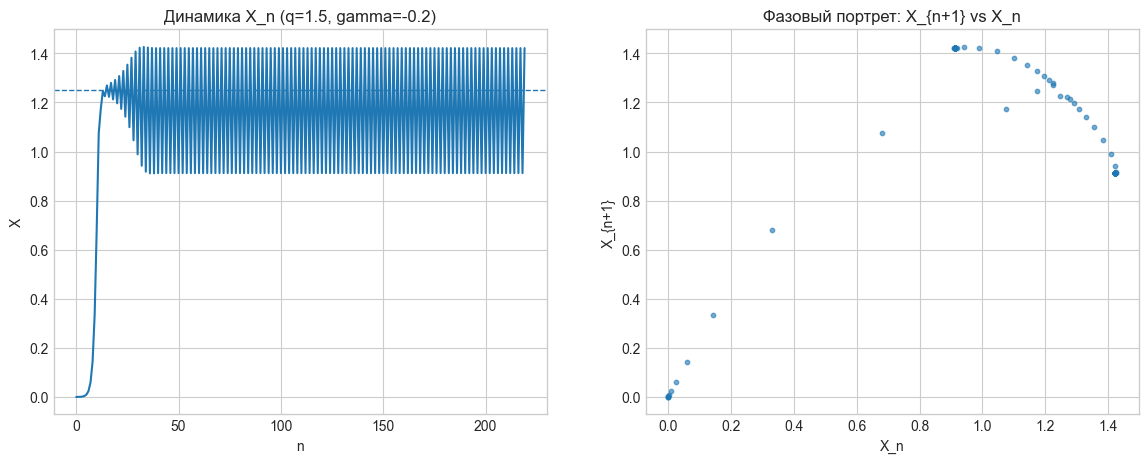
\includegraphics[keepaspectratio]{src/mixed_neg/dyn_phas_q15_gm02.png}}

\subsection{Зона деградации интерпретации}
\label{sec:zona-degradatsii-interpretatsii}

При росте интенсивности или при усилении памяти смешанная модель быстро входит в режимы, где формальная подгонка перестаёт быть содержательной. Для репрезентативного случая \(\gamma=0.5\), \(q=3.5\) траектория вырождается, фазовый портрет теряет регулярную структуру, а регрессионная идентификация становится неинформативной. Аналогичный эффект возникает и при достаточно сильной отрицательной памяти, когда стимулирующий вклад предыстории сочетается с сужением области устойчивости.

Особенно важно, что порог \(\gamma=-1\) задаёт границу интерпретации стационарного состояния в принятой нормировке. При \(\gamma<-1\) величина \(X^*\) становится отрицательной, и такие режимы следует трактовать как режимы, плохо интерпретируемые в данной нормировке, а не как обычные экономические траектории роста.

\begin{figure}[htbp]
\centering
\pandocbounded{\includegraphics[keepaspectratio,alt={dyn\_phas\_35}]{src/mixed/dyn_phas_35.png}}
\caption{dyn\_phas\_35}
\end{figure}

\subsection{Итоговая таблица по смешанной модели}
\label{sec:itogovaya-tablitsa-po-smeshannoi-modeli}

{\def\LTcaptype{none} % do not increment counter
\begin{longtable}[]{@{}
  >{\raggedright\arraybackslash}p{(\linewidth - 8\tabcolsep) * \real{0.2000}}
  >{\raggedright\arraybackslash}p{(\linewidth - 8\tabcolsep) * \real{0.2000}}
  >{\raggedright\arraybackslash}p{(\linewidth - 8\tabcolsep) * \real{0.2000}}
  >{\raggedright\arraybackslash}p{(\linewidth - 8\tabcolsep) * \real{0.2000}}
  >{\raggedright\arraybackslash}p{(\linewidth - 8\tabcolsep) * \real{0.2000}}@{}}
\toprule\noalign{}
\begin{minipage}[b]{\linewidth}\raggedright
Знак \(\gamma\)
\end{minipage} & \begin{minipage}[b]{\linewidth}\raggedright
Экономический смысл памяти
\end{minipage} & \begin{minipage}[b]{\linewidth}\raggedright
Знак коэффициента при \(Lag_1\)
\end{minipage} & \begin{minipage}[b]{\linewidth}\raggedright
Устойчивость
\end{minipage} & \begin{minipage}[b]{\linewidth}\raggedright
Тип сбоя интерпретации
\end{minipage} \\
\midrule\noalign{}
\endhead
\bottomrule\noalign{}
\endlastfoot
\(\gamma>0\) & память усиливает ограничение & отрицательный & область устойчивости сужается при росте \(q\) & при высокой интенсивности возникает вырождение траектории и теряется информативность прогноза \\
\(\gamma<0\), \(-1<\gamma<0\) & память расширяет потенциал развития & положительный & устойчивость становится более хрупкой & при усилении памяти и \(q\) возникает деградационный режим и срыв идентификации \\
\(\gamma\le -1\) & режим плохо интерпретируем в данной нормировке & формально положительный, но содержательно нестабилен & стационарное состояние теряет осмысленность & регрессионные коэффициенты перестают иметь экономическую интерпретацию \\
\end{longtable}
}

\subsection{Выводы по смешанной модели}
\label{sec:vyvody-po-smeshannoi-modeli}

Смешанная модель выступает кульминацией основной части главы. Во-первых, она показывает, что регрессия в принципе способна различать совместное действие текущего уровня и памяти. Во-вторых, знак \(\gamma\) меняет не только устойчивость системы, но и экономический смысл лагового эффекта. В-третьих, именно здесь наиболее ясно проявляется граница интерпретируемости: при усилении памяти и росте интенсивности формальная подгонка быстро теряет содержательную ценность, а траектория переходит в деградационный режим.

\subsection{Дополнение: смешанная модель на коротких выборках (стадии + скользящие окна)}
\label{sec:dopolnenie-smeshannaya-model-na-korotkih-vyborkah-stadii-skolzyaschie-okna}

\subsubsection{Короткие окна как тест двухфакторной структуры}
\label{sec:korotkie-okna-kak-test-dvuhfaktornoi-struktury}

Этот блок нужен как локальная проверка главного результата смешанной модели: сохраняется ли на коротких окнах одновременная идентификация \(X_n\) и \(Lag_1\), и что разрушается первым при усложнении динамики.

Используются скользящие окна длины 25 и лаговое пространство до 10. В отличие от базовой и delay-модели здесь проверяется уже не один доминирующий фактор, а двухфакторная структура и знак лагового эффекта.

\pandocbounded{\includegraphics[keepaspectratio]{src/mixed_interval/1.png}}

\subsubsection{Тест 1. Сохраняется ли двухфакторная структура?}
\label{sec:test-1-sohranyaetsya-li-dvuhfaktornaya-struktura}

В устойчивом режиме при \(\gamma>0\) и умеренном \(q\) короткие окна в целом сохраняют правильную структуру: на информативных фрагментах коэффициенты при \(X_n\) и \(Lag_1\) остаются близкими к теоретическим значениям \(-q\) и \(-q\gamma\). Это означает, что локальное окно в принципе не уничтожает возможность распознать смешанную природу процесса.

Однако уже в устойчивой зоне список переменных \texttt{STEPWISE} оказывается менее надёжным, чем в базовой и delay-модели: при выходе на плато лаги становятся взаимозаменяемыми, и память начинает распределяться по нескольким предикторам. Поэтому для mixed-модели короткое окно следует читать прежде всего по \texttt{ENTER}, \(\beta\) и агрегированному лаговому эффекту, а не по буквальному списку выбранных лагов.

\subsubsection{Тест 2. Что ломается при сложной динамике?}
\label{sec:test-2-chto-lomaetsya-pri-slozhnoi-dinamike}

В циклическом и более сложном режимах короткие окна ещё могут локально удерживать ядро структуры \(X_n + Lag_1\), но интерпретируемость падает быстрее, чем в предыдущих моделях. Ложные лаги появляются раньше, а \texttt{STEPWISE} начинает смешивать физические предикторы с локальными статистическими дублёрами. При дальнейшем усложнении режима окно быстро становится вырожденным: коэффициенты теряют устойчивость, а сама процедура отбора может перестать возвращать модель.

Именно здесь наиболее ясно проявляется главный риск mixed-модели на коротких окнах: первой разрушается не формальная подгонка, а интерпретируемость лаговой структуры.

\subsubsection{Тест 3. Видна ли на окнах смена знака памяти?}
\label{sec:test-3-vidna-li-na-oknah-smena-znaka-pamyati}

В устойчивом режиме при \(\gamma<0\) короткие окна по-прежнему позволяют распознать двухфакторную структуру, но теперь лаговый эффект меняет знак. Это наиболее важный локальный результат для стимулирующей памяти: окно фиксирует не только присутствие памяти, но и изменение её экономического смысла.

При усилении отрицательной памяти устойчивость окна быстро падает. Число информативных фрагментов сокращается, а регрессионные оценки становятся нестабильными. Следовательно, mixed-модель подтверждает общий вывод главы: короткие окна не уничтожают возможность локальной идентификации, но резко ухудшают интерпретируемость при усложнении динамики.

{\def\LTcaptype{none} % do not increment counter
\begin{longtable}[]{@{}
  >{\raggedright\arraybackslash}p{(\linewidth - 8\tabcolsep) * \real{0.2000}}
  >{\raggedright\arraybackslash}p{(\linewidth - 8\tabcolsep) * \real{0.2000}}
  >{\raggedright\arraybackslash}p{(\linewidth - 8\tabcolsep) * \real{0.2000}}
  >{\raggedright\arraybackslash}p{(\linewidth - 8\tabcolsep) * \real{0.2000}}
  >{\raggedright\arraybackslash}p{(\linewidth - 8\tabcolsep) * \real{0.2000}}@{}}
\toprule\noalign{}
\begin{minipage}[b]{\linewidth}\raggedright
Тест
\end{minipage} & \begin{minipage}[b]{\linewidth}\raggedright
Истинная структура
\end{minipage} & \begin{minipage}[b]{\linewidth}\raggedright
Что видно на окнах
\end{minipage} & \begin{minipage}[b]{\linewidth}\raggedright
Что разрушается первым
\end{minipage} & \begin{minipage}[b]{\linewidth}\raggedright
Как интерпретировать
\end{minipage} \\
\midrule\noalign{}
\endhead
\bottomrule\noalign{}
\endlastfoot
Устойчивый режим, \(\gamma>0\) & \(X_n + Lag_1\) & оба фактора читаются & список лагов \texttt{STEPWISE} & опираться на \texttt{ENTER}, \(\beta\), \(B_\Sigma\) \\
Сложная динамика, \(\gamma>0\) & \(X_n + Lag_1\) & ядро частично сохраняется & интерпретируемость лаговой структуры & считать ложные лаги признаком ухудшения окна \\
Устойчивый режим, \(\gamma<0\) & \(X_n + Lag_1\), \(B(Lag_1)>0\) & сохраняется двухфакторность и виден знак памяти & устойчивость окна при усилении памяти & использовать знак лагового коэффициента как диагностический признак \\
\end{longtable}
}

Таким образом, short-window детализация mixed-модели завершает линию сравнения трёх семейств. В базовой модели окно главным образом подтверждает роль \(X_n\), в delay-модели --- роль \(Lag_1\), а в mixed-модели оно способно удерживать двухфакторную структуру только в информативных режимах. При усложнении динамики именно mixed-модель быстрее всего переходит от идентификации к проблеме интерпретируемости.

\subsection{Введение к серии дополнительных экспериментов 2.4.1-2.4.3}
\label{sec:vvedenie-k-serii-dopolnitelnyh-eksperimentov-2-4-1-2-4-3}

Серия дополнительных экспериментов была нужна для того, чтобы уточнить границы применимости короткого окна. После основного анализа стало ясно, что высокая подгонка сама по себе ещё не гарантирует корректную структурную интерпретацию, а ложные лаги, дрейф коэффициентов и вырождение окна могут иметь различную природу. Поэтому в бакалаврской версии работы из всей исследовательской программы оставлены только три укрупнённых результата: сопоставление direct и regression, диагностика режима и интерпретируемости окна, а также сравнение основных контуров анализа с краткими проверками устойчивости.

Подробные parameter sweeps, расширенные таблицы метрик и полные серии однотипных графиков по дополнительным экспериментам вынесены в приложения.

\subsection{Сопоставление прямой идентификации параметров отображения и структурной регрессии}
\label{sec:sopostavlenie-pryamoi-identifikatsii-parametrov-otobrazheniya-i-strukturnoi-regressii}

Первый эксперимент отвечал на вопрос, можно ли заменить регрессионный контур прямой локальной идентификацией параметров отображения. Для базовой модели параметры восстанавливались по минимальному блоку из трёх точек, для модели с запаздыванием --- по четырём точкам, для смешанной модели --- по короткому блоку с локальным решением системы для \(X_n\) и \(X_{n-1}\). В качестве сопоставимого контура использовалась структурная регрессия по теоретически правильным регрессорам на окне длины \(25\).

Проверка гипотезы в рамках вычислительного эксперимента показала, что на чистых траекториях direct-подход действительно может выступать локальным structural probe. Для базовой и delay-модели он воспроизводит структуру закона в пределах вычислительной точности, а для mixed-модели иногда лучше улавливает геометрию редких информативных фрагментов. Однако даже слабый шум быстро делает его менее устойчивым, чем регрессия. На рисунке ниже это видно по росту ошибки главного параметра в зависимости от уровня шума.

\pandocbounded{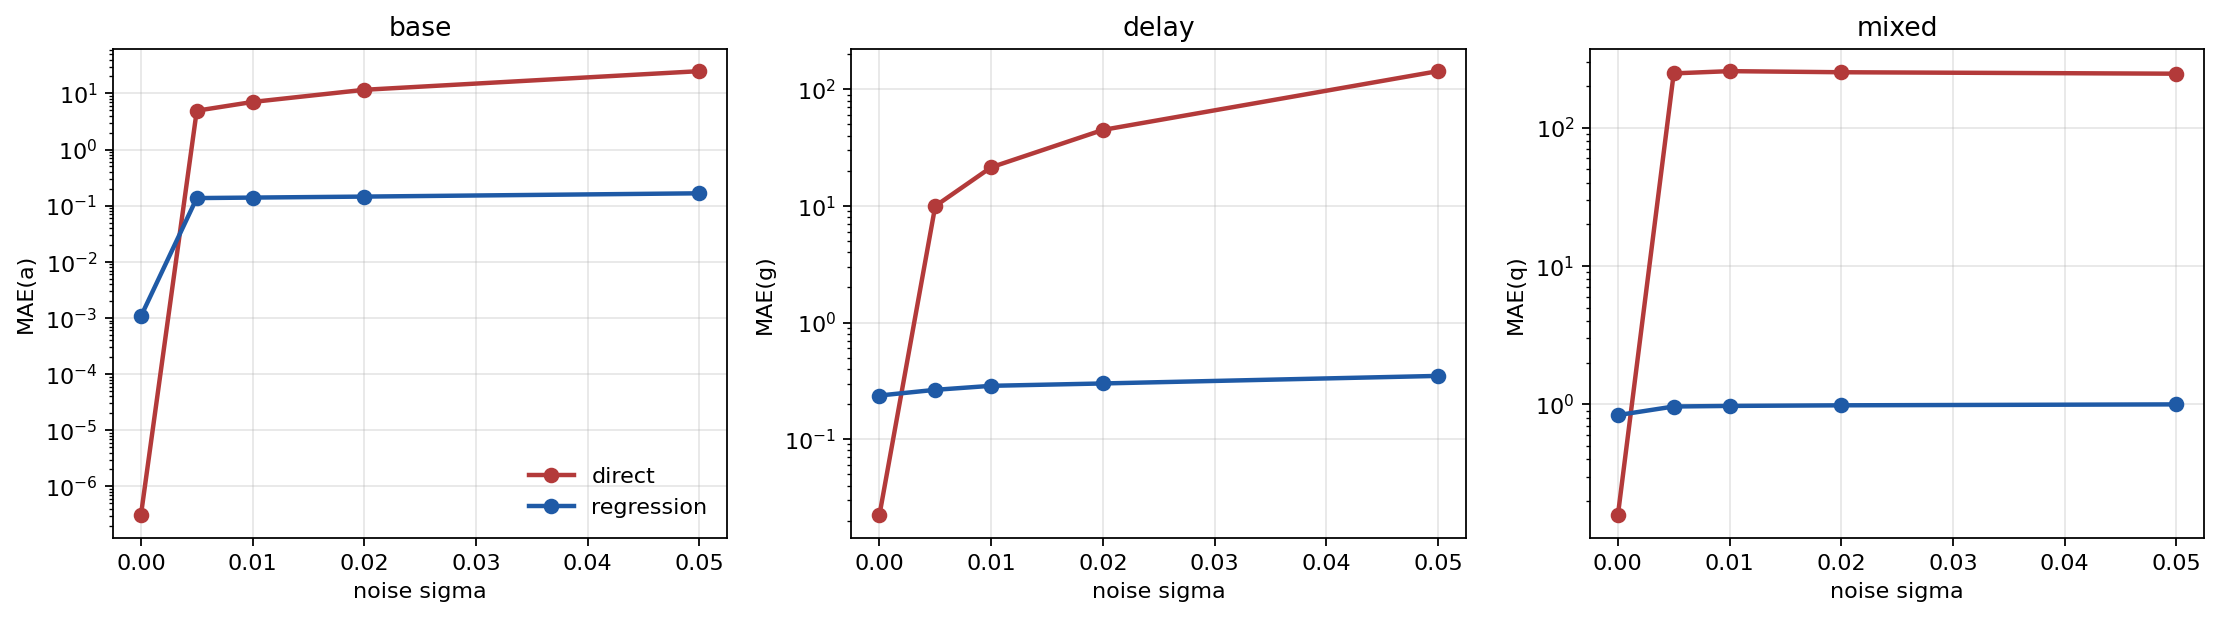
\includegraphics[keepaspectratio]{outputs/planA/planA_noise_sweep_mae.png}}

Главный вывод здесь состоит в том, что прямая идентификация полезна не как замена regression, а как локальный диагностический контур. Она помогает проверить форму закона и момент вырождения окна, но не обеспечивает устойчивого чтения параметров на шумных данных.

\subsection{Диагностика режима и границы интерпретируемости короткого окна}
\label{sec:diagnostika-rezhima-i-granitsy-interpretiruemosti-korotkogo-okna}

Второй укрупнённый результат связан с вопросом, когда короткое окно вообще допускает содержательное чтение. Здесь были сведены вместе режимная диагностика, эксперименты по длине окна, сравнению \(B\)- и \(\beta\)-коэффициентов, а также проверки локальной дисперсии и кондиционности лагового пространства.

Прежде всего оказалось, что выбор инструмента нельзя начинать с регрессии как таковой. Сначала требуется определить тип режима: монотонный, циклический, переходный или вырожденный. Только после этого имеет смысл проверять само окно на интерпретируемость. Показано, что длина окна действительно важна, но не решает проблему автоматически. Более длинное окно уменьшает влияние случайной геометрии и снижает долю ложных лагов, однако не устраняет содержательную мультиколлинеарность. В проблемных окнах ранжирование по \(|\beta|\) обычно устойчивее, чем по \(|B|\), поскольку стандартизация частично компенсирует различие масштабов. Вместе с тем и этот выигрыш работает только там, где окно сохраняет ненулевую локальную дисперсию сигнала.

{\def\LTcaptype{none} % do not increment counter
\begin{longtable}[]{@{}
  >{\raggedright\arraybackslash}p{(\linewidth - 4\tabcolsep) * \real{0.3333}}
  >{\raggedright\arraybackslash}p{(\linewidth - 4\tabcolsep) * \real{0.3333}}
  >{\raggedright\arraybackslash}p{(\linewidth - 4\tabcolsep) * \real{0.3333}}@{}}
\toprule\noalign{}
\begin{minipage}[b]{\linewidth}\raggedright
Фактор
\end{minipage} & \begin{minipage}[b]{\linewidth}\raggedright
Основной вывод
\end{minipage} & \begin{minipage}[b]{\linewidth}\raggedright
Практический смысл
\end{minipage} \\
\midrule\noalign{}
\endhead
\bottomrule\noalign{}
\endlastfoot
Режим окна & тип динамики должен быть определён до выбора регрессии & сначала классифицируется режим, затем выбирается контур чтения \\
Длина окна & Более длинное окно снижает долю артефактов, но не гарантирует правильную структуру & окно нужно увеличивать осмысленно, а не механически \\
\(|\beta|\) против \(|B|\) & \(\beta\) полезнее в проблемных окнах & ранжирование факторов лучше вести по стандартизованным коэффициентам \\
Локальная дисперсия & Падение \(Var(\omega)\) лишает окно структурного сигнала & такие окна не следует читать как память \\
Кондиционность & Высокая \(\kappa(\widetilde{X})\) усиливает ложные лаги & перед чтением лагов нужна геометрическая проверка \\
\end{longtable}
}

Тем самым короткое окно может оказаться неинтерпретируемым по двум разным причинам: либо из него исчезает локальный сигнал, либо лаговое пространство становится практически взаимозаменяемым. В первом случае речь идёт о low-dispersion окнах, во втором --- о collinearity-heavy окнах. Именно поэтому высокий fit не тождествен интерпретируемости, а режимная диагностика должна предшествовать регрессионному чтению.

\subsection{Сравнение основных контуров анализа и проверки устойчивости}
\label{sec:sravnenie-osnovnyh-konturov-analiza-i-proverki-ustoichivosti}

Третий укрупнённый результат относится уже к выбору инструмента внутри допущенного окна. Для этого были сопоставлены ENTER и STEPWISE, агрегированный показатель памяти \(B_\Sigma\), а также краткие контрольные проверки устойчивости через Lasso, Ridge, Elastic Net, PCA и настройку \(p\)-порога.

Здесь был получен простой и важный результат. Lasso лучше очищает простую разреженную структуру, STEPWISE чаще удерживает конкурирующие содержательные факторы в mixed-режимах, ENTER и Ridge полезны как плотные референсные модели, а PCA и настройка \(p\)-порога выступают лишь как контрольные проверки устойчивости. Иными словами, ни один из этих методов не заменяет предварительную режимную диагностику и фильтр интерпретируемости, а лишь уточняет чтение уже допущенного окна.

{\def\LTcaptype{none} % do not increment counter
\begin{longtable}[]{@{}
  >{\raggedright\arraybackslash}p{(\linewidth - 4\tabcolsep) * \real{0.3333}}
  >{\raggedright\arraybackslash}p{(\linewidth - 4\tabcolsep) * \real{0.3333}}
  >{\raggedright\arraybackslash}p{(\linewidth - 4\tabcolsep) * \real{0.3333}}@{}}
\toprule\noalign{}
\begin{minipage}[b]{\linewidth}\raggedright
Контур
\end{minipage} & \begin{minipage}[b]{\linewidth}\raggedright
Сильная сторона
\end{minipage} & \begin{minipage}[b]{\linewidth}\raggedright
Ограничение
\end{minipage} \\
\midrule\noalign{}
\endhead
\bottomrule\noalign{}
\endlastfoot
STEPWISE & сохраняет competing true factors & чувствителен к ложным включениям \\
Lasso & очищает простую структуру & может терять часть истинной памяти \\
ENTER / Ridge & дают плотный референс & плохо подходят для окончательной интерпретации \\
PCA & диагностирует численную вырожденность & не даёт содержательной замены исходным лагам \\
\(p\)-tuning & настраивает жёсткость отбора & не устраняет геометрию ложных лагов \\
\end{longtable}
}

Таким образом, Lasso, PCA и настройка \(p\)-value не образуют самостоятельных методологических направлений. Их роль состоит в проверке устойчивости главного вывода: никакая локальная статистическая настройка не заменяет режимную диагностику и фильтр интерпретируемости окна.

\subsection{Итоговая схема интерпретации результатов}
\label{sec:itogovaya-shema-interpretatsii-rezultatov}

По итогам дополнительных экспериментов маршрут анализа короткого окна можно записать в виде четырёх шагов.

\begin{enumerate}
\def\labelenumi{\arabic{enumi}.}
\tightlist
\item
  Сначала определяется режим процесса и решается вопрос, уместен ли регрессионный контур.
\item
  Затем проверяются локальная дисперсия сигнала и геометрия лагового пространства.
\item
  После этого выбирается контур чтения: direct-probe, структурная регрессия, агрегированный показатель памяти или отказ от интерпретации.
\item
  Только на последнем этапе интерпретируются коэффициенты, их знаки и относительная значимость факторов.
\end{enumerate}

Главный результат серии 2.4.1-2.4.3 состоит в переходе от универсальной эконометрической интерпретации к режимно-зависимой процедуре анализа. В нелинейной динамике качество подгонки, численная устойчивость и физическая интерпретируемость не совпадают и потому должны оцениваться раздельно.

\section{ЗАКЛЮЧЕНИЕ И ОБЩИЕ ВЫВОДЫ ПО РЕЗУЛЬТАТАМ МОДЕЛИРОВАНИЯ}
\label{sec:zaklyuchenie-i-obschie-vyvody-po-rezultatam-modelirovaniya}

\subsection{Общий вывод главы}
\label{sec:obschii-vyvod-glavy}

В рамках проведённого вычислительного эксперимента получены пять основных выводов.

\begin{enumerate}
\def\labelenumi{\arabic{enumi}.}
\tightlist
\item
  Линейная регрессия способна надёжно восстанавливать структурную форму темпа прироста на длинных траекториях и в информативных режимах короткого окна.
\item
  Ложные лаги появляются прежде всего в циклических, переходных и геометрически вырожденных окнах, а не только как дефект конкретного алгоритма отбора.
\item
  Высокий fit не равен хорошей интерпретации: окно может хорошо подгоняться и одновременно не допускать содержательного чтения коэффициентов.
\item
  Короткие окна полезны как инструмент локальной диагностики, но требуют предварительной проверки режима, локальной дисперсии и кондиционности лагового пространства.
\item
  Главный результат synthetic-части состоит в построении маршрута анализа, который затем переносится на реальные данные: сначала режим, затем интерпретируемость, затем выбор контура и только после этого чтение коэффициентов.
\end{enumerate}

Таким образом, глава 2 показывает не ``лучшую регрессию вообще'', а условия, при которых регрессионный анализ в нелинейной динамике остаётся содержательно допустимым.

\subsection{Ограничения главы 2}
\label{sec:ogranicheniya-glavy-2}

Полученные результаты следует интерпретировать с учётом ограничений проведённого исследования.

\begin{enumerate}
\def\labelenumi{\arabic{enumi}.}
\tightlist
\item
  Эксперименты проводились на synthetic-данных, где закон генерации задавался заранее и потому исследование велось в контролируемых условиях.
\item
  Рассматривался ограниченный набор дискретных нелинейных моделей: базовая, запаздывающая и смешанная.
\item
  В части экспериментов использовались чистые траектории или простые схемы шума, что не исчерпывает разнообразия реальных возмущений.
\item
  Результаты зависят от длины окна, выбранного лагового пространства и конкретной конфигурации режимов, поэтому их следует переносить на эмпирику как методологический маршрут, а не как готовый набор универсальных численных порогов.
\end{enumerate}

Эти ограничения не отменяют полученных выводов, но задают корректные границы их применения и непосредственно подводят к главе 3, где построенный маршрут проверяется уже на реальных данных.

